\begin{ex} %Câu 41
Cho hàm số $y=f( x )$ có bảng biến thiên như sau:
 \\ \centerline{
\begin{tikzpicture}
\tkzTabInit[nocadre,lgt=1.2,espcl=2.2]
{$x$ /.6,$f'(x)$ /.6,$f(x)$ /1.5}
{$-\infty$,$0$,$3$,$+\infty$}
\tkzTabLine{,+,$0$,-,$0$,+,}
\tkzTabVar{-/ $-\infty$ ,+/$2$,-/$1$,+/$+\infty$}
\end{tikzpicture}
}\\
Số nghiệm thực phân biệt của phương trình $f'( f( f( x ) ) )=0$ là
\choice 
{ $5$}
{ $3$}
{ $4$}
{ \True $2$} \end{ex} 
\begin{ex} %Câu 47
Cho hàm số $y=f(x)$ có đạo hàm là $f^\prime(x)=x^2-82x,\,\forall x \in \mathbb{R}$ . Có bao nhiêu giá trị nguyên dương của tham số $m$  để hàm số $y=f(x^4-18x^2+m)$ có đúng $7$ điểm cực trị?
\choice 
{ $83$ }
{ vô số}
{ \True $80$ }
{ $81$} \end{ex}
\Closesolutionfile{ans}
\begin{ex} %{Cau 1}

\choice
{}
{}
{}
{}
\end{ex}

\begin{ex} %{Cau 2}

\choice
{}
{}
{}
{}
\end{ex}

\begin{ex} %{Cau 3}

\choice
{}
{}
{}
{}
\end{ex}

\begin{ex} %{Cau 4}

\choice
{}
{}
{}
{}
\end{ex}

\begin{ex} %{Cau 5}

\choice
{}
{}
{}
{}
\end{ex}

\begin{ex} %{Cau 6}

\choice
{}
{}
{}
{}
\end{ex}

\begin{ex} %{Cau 7}

\choice
{}
{}
{}
{}
\end{ex}

\begin{ex} %{Cau 8}

\choice
{}
{}
{}
{}
\end{ex}

\begin{ex} %{Cau 9}

\choice
{}
{}
{}
{}
\end{ex}

\begin{ex} %{Cau 10}

\choice
{}
{}
{}
{}
\end{ex}

\begin{ex} %{Cau 11}

\choice
{}
{}
{}
{}
\end{ex}

\begin{ex} %{Cau 12}

\choice
{}
{}
{}
{}
\end{ex}

\begin{ex} %{Cau 13}

\choice
{}
{}
{}
{}
\end{ex}

\begin{ex} %{Cau 14}

\choice
{}
{}
{}
{}
\end{ex}

\begin{ex} %{Cau 15}

\choice
{}
{}
{}
{}
\end{ex}

\begin{ex} %{Cau 16}

\choice
{}
{}
{}
{}
\end{ex}

\begin{ex} %{Cau 17}

\choice
{}
{}
{}
{}
\end{ex}

\begin{ex} %{Cau 18}

\choice
{}
{}
{}
{}
\end{ex}

\begin{ex} %{Cau 19}

\choice
{}
{}
{}
{}
\end{ex}

\begin{ex} %{Cau 20}

\choice
{}
{}
{}
{}
\end{ex}

\begin{ex} %{Cau 21}

\choice
{}
{}
{}
{}
\end{ex}

\begin{ex} %{Cau 22}

\choice
{}
{}
{}
{}
\end{ex}

\begin{ex} %{Cau 23}

\choice
{}
{}
{}
{}
\end{ex}

\begin{ex} %{Cau 24}

\choice
{}
{}
{}
{}
\end{ex}

\begin{ex} %{Cau 25}

\choice
{}
{}
{}
{}
\end{ex}
\begin{ex} %{Cau 26}

\choice
{}
{}
{}
{}
\end{ex}
\begin{ex} %{Cau 27}

\choice
{}
{}
{}
{}
\end{ex}
\begin{ex} %{Cau 28}

\choice
{}
{}
{}
{}
\end{ex}
\begin{ex} %{Cau 29}

\choice
{}
{}
{}
{}
\end{ex}
\begin{ex} %{Cau 30}

\choice
{}
{}
{}
{}
\end{ex}
\begin{ex} %{Cau 31}

\choice
{}
{}
{}
{}
\end{ex}
\begin{ex} %{Cau 32}

\choice
{}
{}
{}
{}
\end{ex}
\begin{ex} %{Cau 33}

\choice
{}
{}
{}
{}
\end{ex}
\begin{ex} %{Cau 34}

\choice
{}
{}
{}
{}
\end{ex}
\begin{ex} %{Cau 35}

\choice
{}
{}
{}
{}
\end{ex}
\begin{ex} %{Cau 36}

\choice
{}
{}
{}
{}
\end{ex}
\begin{ex} %{Cau 37}

\choice
{}
{}
{}
{}
\end{ex}
\begin{ex} %{Cau 38}

\choice
{}
{}
{}
{}
\end{ex}
\begin{ex} %{Cau 39}

\choice
{}
{}
{}
{}
\end{ex}
\begin{ex} %{Cau 40}

\choice
{}
{}
{}
{}
\end{ex}
